\documentclass[12pt,a4paper, flushleft]{article}
\usepackage[utf8]{inputenc}
\usepackage{amsmath,amssymb,amsthm}
\usepackage[T2A]{fontenc}
\usepackage[russian]{babel}
\usepackage{mathrsfs, dsfont} % специальные шрифты, по типу \mathscr или \dsfont
\usepackage{comment} %для многострочных комментариев
\usepackage{xcolor} %для гиперссылок в тексте и их цвета
\usepackage{hyperref}
\usepackage{graphicx}
\usepackage{wrapfig}
\usepackage{lipsum}
\usepackage{multicol}
\graphicspath{/home/cowberry/Documents/10M/SPTYM/pics/}
\usepackage[left=2cm,right=2cm,top=2cm,bottom=2cm]{geometry}	
\usepackage[most]{tcolorbox}
\definecolor{block-gray}{gray}{0.90} % уровень прозрачности (1 - максимум)
\newtcolorbox{myquote}{colback=block-gray,grow to right by=-25mm,grow to left by=-25mm, boxrule=1pt,boxsep=0pt,breakable}
\author{Анатолий Коченюк, команда ЛНМО\#2}
\date{Март 2019}
\title{Зодача \textsuperscript{\textregistered} №5}
\newcommand{\horline}[1]{
		\begin{center}
			\begin{picture}(#1, 2)
				\line(1,0){#1}%
			\end{picture}
		\end{center}
	}
\title{
	\vspace{4cm}	
	\horline{380}	
	\begin{center}
		\begin{Huge}
			\textbf{\emph{Задача 4. Поймай меня, если сможешь}}
		\end{Huge}
	\end{center}	
	\vspace{-1.3cm}	
	\horline{400}
	%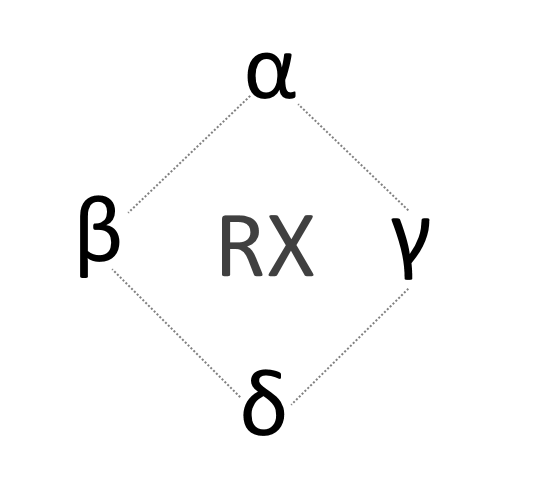
\includegraphics[scale=0.15]{abgrx.png}
}
\newtheorem{Def}{Определение}[section]
\newtheorem{Th}{Теорема}[section]
\newtheorem{Lm}{Лемма}[section] 
\newtheorem{Pb}{Задача}[section]
\newtheorem{Qu}{Признак}[section]
\newtheorem{St}{Утверждение}[section]
\newtheorem{Sl}{Следствие}[section]
\newtheorem{Zm}{Замечание}[section]
\newtheorem{Con}{Условие}[section]
\usepackage{relsize}
\newcommand{\vel}{\mathlarger{\mathlarger{\upsilon}}}
\newcommand{\der}[1]{\overset{\cdot}{#1}}
\newcommand{\dder}[1]{\overset{\cdot \cdot}{#1}}
\newcommand{\Lim}[2]{\lim\limits_{#1\to #2}}
\newcommand{\Ch}[1]{\overset{#1}{=}}
\newcommand{\p}[1]{#1^{\prime}}
\newcommand{\pp}[1]{#1^{\prime\prime}}
\newcommand{\ol}[1]{\overline{#1}}
\newcommand{\oll}[1]{\overline{\overline{#1}}}
\newcommand{\ov}[2]{\overset{#1}{#2}}
\newcommand{\un}[1]{\underline{#1}}
\newcommand{\gr}[2]{\includegraphics[scale=#1]{../pics/#2}}
\newcommand{\fl}[1]{\lfloor #1 \rfloor}
\usepackage{comment}

\begin{document}
\maketitle
\pagebreak
\section{Считающие функции}

\begin{Def}
	Назовём функцию считающей, если её можно представить в виде $$h(x) = c_1\fl x + c_2 \fl{x/2} + c_3 \fl{x/3} + \dots$$
	где $c_1, c_2\dots$ -- целочисленные коэффициенты, а $\fl x$ -- целая часть $x$
	
	Далее $h(x)$ -- считающая функция
\end{Def}

\subsection{Равенство целой части и образа считающей функции}
\begin{Th}
	$\fl x = \fl y \Rightarrow h(x) = h(y)$
\end{Th}
\begin{proof}
	Если целые части равны, то $x, y$ можно представить следующим образом:
	
	$x = z + w_x\quad y = z + w_y$, где $z$ -- целая часть $x$ и $y$, а $w_x, w_y<1$ -- их дробные части 
	
	Для доказательства теоремы будет достаточно условия $\forall n \fl{x/n} = \fl{y/n}$
	
	Или, что то же самое $\forall n \fl{z/n + w_x/n} = \fl{z/n + w_y/n}$
	
	Рассмотрим случай, когда $n = 2$
	
	$\fl{z/2 + w_x/2} = \fl{z/2 + w_y/2}$
	
	т.к. $z$ -- целое, то может быть два случая:
	\begin{enumerate}
		\item $z/2$ -- целое, а тогда $\fl{z/2 + w_x/2} = \fl{z/2 + w_y/2}$, т.к. вторые слагаемые $<1$
		\item $z/2 = \p z + \dfrac{1}{2}, \p z\in\mathds{Z}$ в таком случае $\fl{z/2 + w_x/2} = \fl{z/2}$, т.к. $w_x/2<\dfrac{1}{2}$ аналогично $\fl{z/2 + w_y} = \fl{z/2}\Rightarrow \fl{z/2 + w_x/2} = \fl{z/2 + w_y/2}$
	\end{enumerate}
	
	А значит в любом случае $\fl{z/2 + w_x/2} = \fl{z/2 + w_y/2}$
	
	Теперь рассмотрим произвольное $n$.
	
	Здесь аналогично может быть $n$ случаев $z/n$ -- целое $\p z +  \dfrac{i}{n}, i = \overline{0, n-1}$, но $w_x/n, w_y/n <1/n$ и аналогчно случаю с $n=2$ не могут повлиять на целую часть.
	
	А значит $\forall n\, \fl{x/n} = \fl{y/n}$, т.е. все элементы $h(x)$ и $h(y)$ равны, а значит $h(x) = h(y)$
\end{proof}

\subsection{$h(n) - h(n-1)$}

$n\in\mathds{Z}$

$h(n) = c_1\fl n + c_2 \fl{n/2} + c_3 \fl{n/3} + \dots$

$h(n-1) = c_1\fl {n-1} + c_2 \fl{n/2 - 1/2} + c_3 \fl{n/3 - 1/3} + \dots$

$\sphericalangle h(n) - h(n-1) = c_1(\fl n - \fl{n-1}) + c_2(\fl{n/2} - \fl{n/2 - 1/2}) + c_3(\fl{n/3} - \fl{n/3 - 1/3}) + \dots = c_1(n-1+1) + c_2()$
\end{document} 
